\section{Durchführung}
\label{sec:Durchführung}

\subsection{Versuchsaufbau}
\label{sec:Versuchsaufbau}
%\begin{figure}
%	\centering
%	\caption{Schematische Darstellung des Versuchsaufbaus \cite{anleitung}.}
%	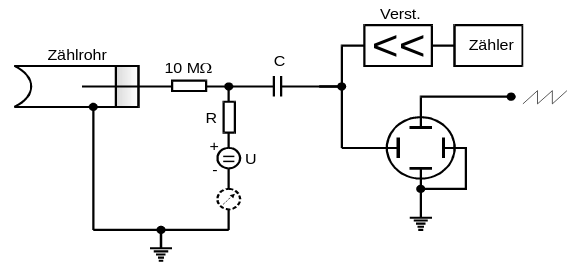
\includegraphics{Bilder/aufbau.png}
%	\label{fig:aufbau}
%\end{figure}
%
%\begin{figure}
%	\centering
%	\caption{Schematische Darstellung der Quelle zur Erzeugung radioaktiven Isotopen \cite{anleitung}.}
%	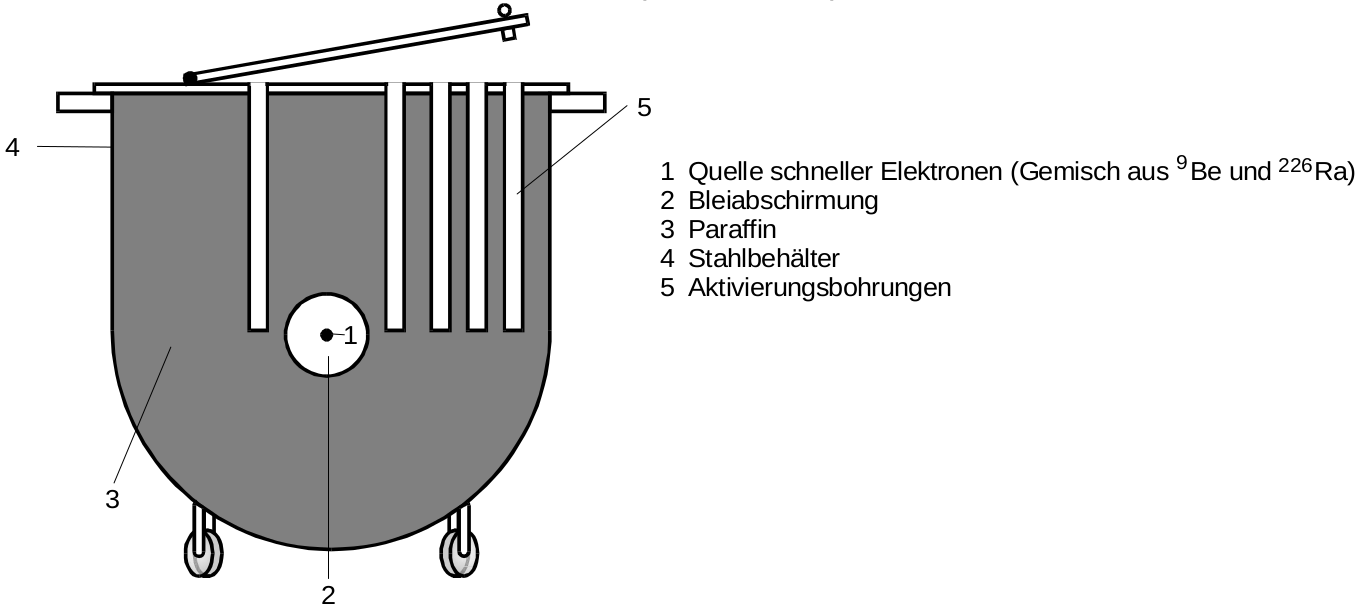
\includegraphics{content/toepfchen.png}
%	\label{fig:kochen}
%\end{figure}
%
Der Versuchsaufbau -- wie in Abbildung \ref{fig:aufbau} dargestellt -- besteht im Wesentlichen 
aus einem zerfallenden radioaktiven Isotop und einem Geiger-Müller-Zählrohr, welches die 
zerfallenden Kerne misst.
Das Geiger-Müller-Zählrohr ist entspricht einer mit Gas gefüllten Röhre. Trifft ein $\beta$-
oder $\gamma$- Teilchen auf ein Gasteilchen wird dieses ionisiert und kann aufgrund einer
anliegenden Spannung an der Röhre gemessen werden.
Dabei werden die gemessenen Zerfälle pro Messzeitintervall, welches am Zeitgeber einstellbar 
ist, an den Zählern 1 und 2 angezeigt. Nach jedem Messvorgang wird der Zähler umgeschaltet und 
der vorherige Wert auf dem aktuellen Zähler wird überschrieben. Der Versuchsaufbau ist mit
einer Blei-Abschirmung ausgestattet um die radioaktive Strahlung abzuschirmen.

Zur Erzeugung der radioaktiven Isotope wird das Objekt in Abbildung \ref{fig:kochen} verwendet.
Hierbei werden stabile Kerne mit niederenergetischen Neutronen beschossen. 
Da die Neutronen ihre Energie durch elastische Stöße an die Kerne übergeben und die maximale
Energie bei gleichen Massen der Stoßpartner erreicht wird, werden die Neutronen in einem 
Paraffinmantel gebremst, bis sie die optimale Energie besitzen.


\subsection{Versuchsbeschreibung}
\label{sec:Versuchsbeschreibung}
Zur Aufnahme der \textbf{Charakteristik des Zählrohrs} wird eine $\beta$-Quelle vor das Endfenster des Zählrohrs gestellt und die Zählrate über ein Intervall von einer Minute in Abhängigkeit zur Betriebsspannung $U$ gemessen.\\
Die Betriebsspannung wird hierbei in Schritten von $\SI{10}{\volt}$ heraufgeregelt.
Da wahrscheinlich ein Defekt im Versuchsaufbau vorliegt, läuft die Messung statt über das Intervall $\SI{350}{\volt}$-$\SI{700}{\volt}$ über das Intervall $\SI{450}{\volt}$ bis $\SI{900}{\volt}$.\\
Zudem wird die Stromstärke $I$ des Zählrohrstrom mittels eines empfindlichen Strommessgeräts zur Untersuchung der pro Teilchen vom Zählrohr freigesetzten Ladungsmenge erfasst.

In einem nur qualitativen Experiment werden werden die \textbf{Nachentladungen} am Oszilloskopschirm sichtbar gemacht.
Dazu wird die $\beta$-Quelle so weit vom Eintrittsfenster des Zählrohrs entfernt, dass lediglich ein Impuls auf dem Bildschirm samt den zugehörigen Nachentladungen zu sehen ist.\\
Es wird das Oszilloskopbild bei geringer Betriebsspannung nahezu ohne auftretende Nachentladungen mit $U=\SI{450}{\volt}$, mit dem Oszilloskopbild mit deutlich sichtbaren Nachentladungen bei einer Betriebsspannung von $U=\SI{700}{\volt}$, verglichen.

Die Untersuchung der \textbf{Totzeit} erfolgt über zwei Methoden.\\
Zum Einen wird sie aus dem Oszilloskopbild bestimmt.
Hierzu wird aus dem Oszilloskopbild die Zeitdifferenz zwischen zwei Impulsen maximaler Höhe bestimmt. Hierzu muss die Strahlungsintensität hoch sein. Die Quelle wird daher nahe vor dem Eintrittsfenster des Zählrohrs platziert.

Zudem wird die Totzeit über die \textbf{Zwei-Quellen-Methode} bestimmt.
Hierzu wird zunächst eine Messung der Impulsrate mit nur einer Quelle über ein Zeitintervall von $\SI{1}{\minute}$ durchgeführt.
Anschließend wird eine zweite Quelle hinzugefügt und die Impulsrate beider Quellen gemeinsam bestimmt. Schließlich wird die zweite Quelle ebenfalls über das gleiche Zeitintervall alleine vermessen.
Es ist darauf zu achten, dass beim Hinzufügen, beziehungsweise Entfernen der Quellen die Position der jeweils andere Quelle bezüglich des Zählrohrs möglichst nicht geändert wird.
